\section{ProgCPP}

    \subsection{Nützliche Links}
        \begin{itemize}
            \item STL: https://en.cppreference.com/
            \item Boost: https://www.boost.org/
            \item Github (Lizenzen beachten!)
        \end{itemize}

    \subsection{Wichtige Kurzbefehle}
        \begin{tabular}{ll}
            \verb|cd "Path"| & Pfad anwählen \\
            \verb|cd ..| & um eine Ebene nach oben (zurück) \\
            \verb|mkdir "Ordnername"| & Ordner erstellen \\
            \verb|rmkdir "Ordnername"| & Ordner löschen \\
            \verb|rm -rf *| & Alles innerhalb vom aktuellen Ordner löschen \\
            \verb|rm "Datei"| & Datei löschen \\
            \verb|mv "Name alt" "Name neu"| & Datei umbenennen \\
            \verb|cp "Datei alt" "Datei neu"| & Datei kopieren und benennen \\
            \verb|clang++ -Wall -o "Outputname" "Inputdatei"| & clang++ - Compiler mit Warnungen \\
            %\verb|clang++ -Wall -o "Outputname" "Inputdatei" -lm| & -lm für Mathebibliothek \\
            \verb|ls| & Listet alle Files im akt. Verzeichnis auf \\
            \verb|ls -l| & Inkl. Informationen wie Grösse u.a. \\
            \verb|ls -a| & Inkl. versteckten Dateien \\
            \verb|ls -al| & Beide Varianten \\
        \end{tabular}

    \subsection{Datentypen}

        \subsubsection{Namen}
            \begin{tabular}{|l|l|l|}
                \hline
                Variablen, Konstanten & Funktionen & Klassen, Strukt., Enums \\
                \hline
                mit Kleinbuchst. beginnen & mit Kleinbuchst. beginnen & mit Grossbuchst. beginnen \\
                camelCase & camelCase & PascalCase \\
                keine Underscores & keine Underscores & keine Underscores \\
                &&\\
                \verb|maxSpeed| & \verb|getCount()| & \verb|MotorController| \\
                \hline
            \end{tabular}

    \subsection{Streams}
        Ein Stream rep. einen Datenstrom, z.B. ein Terminal, Dateien oder Datenverkehr (TCP/IP).

        \textbf{Standardströme:}
        \begin{itemize}
            \item \verb|cin|
            \item \verb|cout|
            \item \verb|cerr|
            \item \verb|clog|
        \end{itemize}

        \verb|cin| und \verb|cout| müssen ganz links in der Zeile stehen!

        \subsubsection{Flags}
            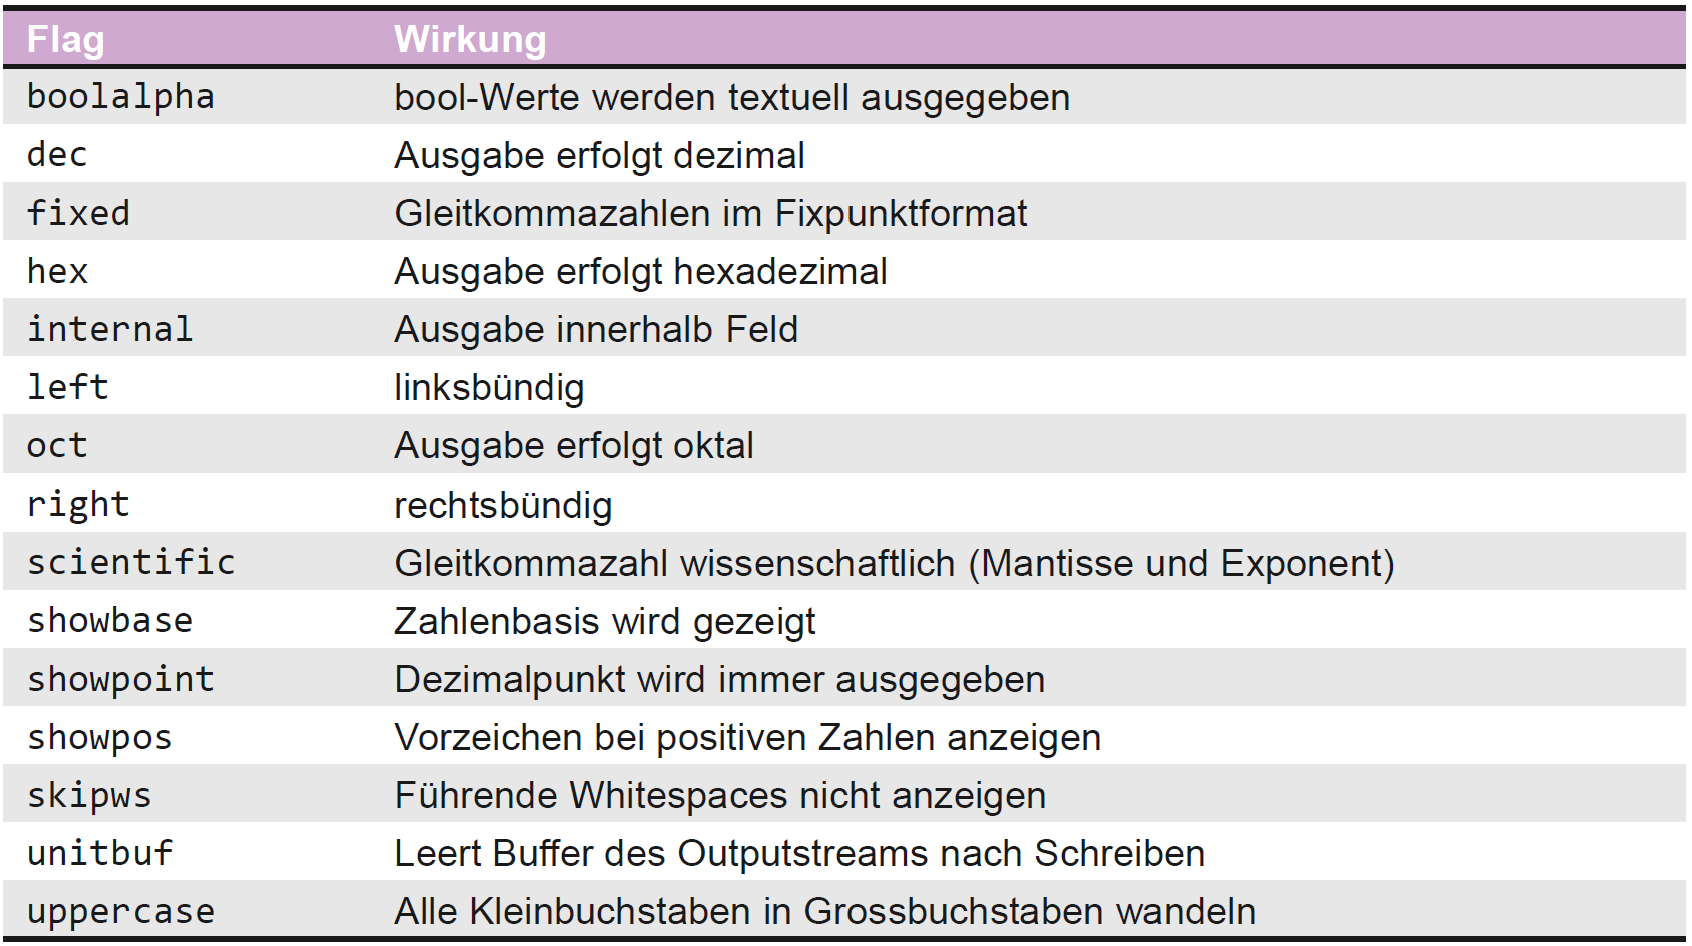
\includegraphics[width=0.95\linewidth]{Bilder/cpp_flags-iostream.png}

    \subsection{Operatoren und Operanden}

        \subsubsection{Logisch vs. bitweise Operatoren}
            $\parallel$ oder \verb|'or'| = OR\\
            \&\& oder \verb|'and'| = AND \\
            \\
            \textbf{Logisch:}
                \begin{lstlisting}[language=C++]
char a = 0;   //bedeutet unwahr
char b = -27; //bedeutet wahr
if(a and b){
cout << "A und B sind wahr" << endl;
}	
                \end{lstlisting}

    \subsection{Code-Snippets}

        \subsubsection{Hello World!}
            \begin{lstlisting}[language=C++]
#include <iostream>
using namespace std;

int main(){
    cout << "Hello World!" << endl;
    return 0;
}
            \end{lstlisting}
